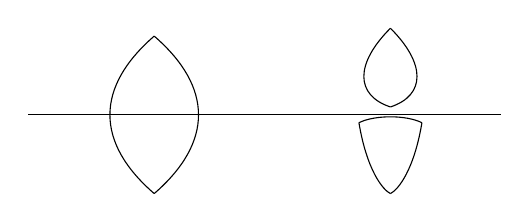
\begin{tikzpicture}
  % horizontal axis line
  \draw (-3.6,0) -- (2.4,0);
  % left: full biconvex lens (vesica) on the axis
  \draw (-2,1) .. controls (-2.75,0.35) and (-2.75,-0.35) .. (-2,-1);
  \draw (-2,1) .. controls (-1.25,0.35) and (-1.25,-0.35) .. (-2,-1);
  % right-top: lens above the axis
  \draw (1,1.1) .. controls (0.55,0.65) and (0.55,0.25) .. (1,0.1);
  \draw (1,1.1) .. controls (1.45,0.65) and (1.45,0.25) .. (1,0.1);
  % right-bottom: cap below the axis (flatter top, curved sides to a point)
  \draw (0.6,-0.1) .. controls (0.7,-0.7) and (0.9,-0.95) .. (1,-1);
  \draw (1.4,-0.1) .. controls (1.3,-0.7) and (1.1,-0.95) .. (1,-1);
  \draw (0.6,-0.1) .. controls (0.8,0.0) and (1.2,0.0) .. (1.4,-0.1);
\end{tikzpicture}
